\documentclass[border=5pt,tikz]{standalone}
\usepackage{amsmath} % for \dfrac
\usepackage{physics}
\usepackage{tikz,pgfplots}
%\usepackage[outline]{contour} % glow around text
\usetikzlibrary{arrows,arrows.meta}
\usetikzlibrary{decorations.markings}
\usetikzlibrary{hobby}
%\usetikzlibrary{pgfplots.fillbetween}
\usepgfplotslibrary{fillbetween}
\tikzset{>=latex} % for LaTeX arrow head
\usepackage{xcolor}


\begin{document}

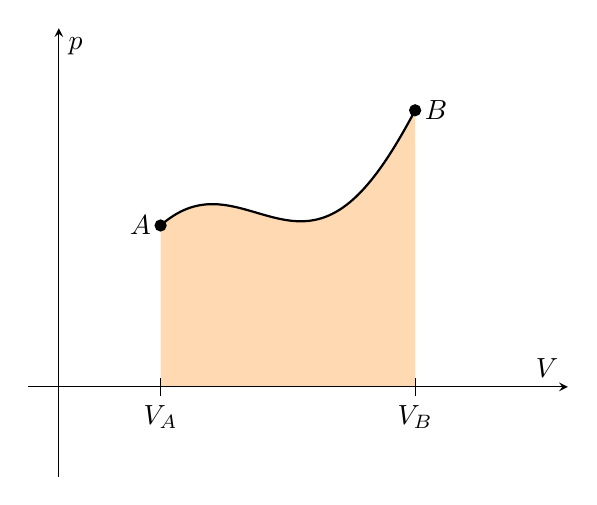
\begin{tikzpicture}
  \begin{axis} [
  	axis lines=center,
    xlabel=$V$,
    ylabel=$p$,
    ticks=none,
    ymin = -0.5,
    ymax = 2,
    xmin = -0.3,
    xmax = 5.0]
    \addplot [name path = A, domain=1:3.5, samples=400, smooth, thick] { 0.4*cos(300*(x-1)/pi) + 0.5*x};
	\filldraw (axis cs:{1}, {0.9}) circle (2pt) node [left] {$A$};
	\filldraw (axis cs:{3.5}, {0.4*cos(300*(3.5-1)/pi) + 0.5*3.5}) circle (2pt) node [right] {$B$};
%        node[pos=0, left] {$A$}; 
    \addplot [name path = B, domain=1:3.5, samples=400, black, thin] {0};
    \addplot [orange, fill opacity=0.3] fill between [of=A and B];
	\draw[] (axis cs:1.0, 0.05) -- (axis cs:1.0, -0.05) node[below] {$V_A$};
	\draw[] (axis cs:3.5, 0.05) -- (axis cs:3.5, -0.05) node[below] {$V_B$};
  \end{axis}
\end{tikzpicture}

\end{document}